\chapter{Lie theory and Jacobi diagrams}
\label{ch:lie-theory-and-jacobi-diagrams}

The fundamental theorem of Vassiliev invariants states that the bialgebra of Vassiliev invariants can be broken up into nice combinatiorial weight systems. So to understand \(\mathcal{V}\) it suffices to understand \(\mathcal{W}\), or equivalently its dual \(\mathcal{A}\). There is a hint that the structure of \(\mathcal{A}\) may relate to Lie algebras.

\begin{mdframed}
	The hint is that Hopf algebras have a lie algebra as their primitive elements \(\mathcal{P}(H)\). However I clearly am confused here, for the following reason. By the Milnor-Moore theorem, applying this to \(\mathcal{A}\), it should be the symmetric algebra (and therefore the universal enveloping algebra, as it's abelian?) of \(\mathcal{P}(\mathcal{A})\).

	However this clashes with my understanding of the raison d'etre of Hinnich-Vaintrob \cite{cyclic-operads-and-the-algebra-of-chord-diagrams}. According to them, the point of their convoluted construction is to realise \(\mathcal{A}\) as the universal enveloping algebra of some Lie algerba. And a key point is that that's not technically true, hence the need to move to more general tensor categroies.

	Further evidence in \cite{noncommutative-chern-weil-theory-and-the-combinatorics-of-wheeling}: ``The STU relation is a formal analogue of the relation in a Universal Enveloping Algebra which equates a commutator with the corresponding bracket'' (the word formal implying that this isn't literally true).

	Page 141 on \cite{introduction-to-vassiliev-invariants} furthermore says that \cite{cyclic-operads-and-the-algebra-of-chord-diagrams} shows \(\mathcal{A}\) (algebra of Jacobi diagrams on the circle) is isomorphic to the center of the universal enveloping algebra of a Casimir Lie algebra in a certain tensor category. Indeed that's my interpretation of HV, but why do if we already know that \(\mathcal{A}\) is already the center (which in this case equals the whole thing) of \(\mathcal{P}(\mathcal{A})\)?!
\end{mdframed}

% TODO: Try to fix(?) and include the below CDM proof of Milnor-Moore
% \begin{theorem}
% 	The bialgebra \(\mathcal{A}\) is canonically isomorphic to the algebra of polynomials in its primitive elements,
% 	\[\mathcal{A} \cong S(\mathcal{P}(\mathcal{A})),\]
% 	where \(S\) denotes the symmetric algebra.
% \end{theorem}
% \begin{proof}
% 	\begin{mdframed}
% 		The proof in \cite{introduction-to-vassiliev-invariants} is readable, but missing crucial details, and containing a typo. Furthermore I cannot find it anywhere else. If there is time, I want to find out if it works and include it. Perhaps compare to the original source.
% 	\end{mdframed}
% \end{proof}

\section{Jacobi diagrams, AS, STU and IHX}

This side of the story reframes the bialgebra \(\mathcal{A}\) as an isomorphic bialgebra known as the algebra of Jacobi diagrams to illuminate the Lie theory connections.

\begin{definition}
	A \textbf{unitrivalent diagram} is a unitrivalent graph (with loops and multiple edges allowed) with the following additional data:
	\begin{itemize}
		\item each trivalent vertex has a fixed cyclic order of incident edge-connections,
		\item the set of univalent vertices has a fixed cyclic order.
	\end{itemize}
	The vector space of unitrivalent diagrams is denoted \(\mathcal{T}\).
\end{definition}

When drawing unitrivalent diagrams, we specify the fixed cyclic order of the univalent edges of a unitrivalent diagram by drawing them connected to a circle. In particular all chord diagrams are Jacobi diagrams with only univalent vertices (the chord ends). Further examples of non-chord diagram Jacobi diagrams would be
\[
	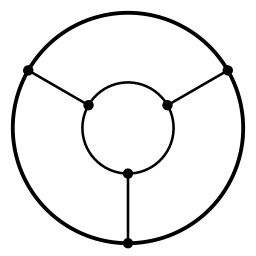
\includegraphics[width=0.13\textwidth, valign=c]{graphics/unitrivalent_diagram_example_1.pdf} \ ,
	\quad
	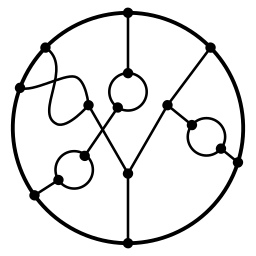
\includegraphics[width=0.13\textwidth, valign=c]{graphics/unitrivalent_diagram_example_2.pdf}
	\in \mathcal{T}.
\]

\begin{definition}
	The \textbf{STU relation} is the relation
		\begin{equation}
			\label{eq:STU}
			\tag{\stu}
			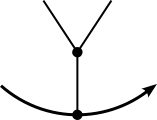
\includegraphics[width=0.10\textwidth, valign=c]{graphics/stu_relation_s.pdf}
			\quad
			=
			\quad
			\includegraphics[width=0.10\textwidth, valign=c]{graphics/stu_relation_t.pdf}
			\quad
			-
			\quad
			\includegraphics[width=0.10\textwidth, valign=c]{graphics/stu_relation_u.pdf}.
		\end{equation}
\end{definition}

As usual, this is not an individual relation but a type of relations, true in any diagrams that are identical except for the subdiagrams being as shown.

Note that the for the chord diagrams inside the algebra of Jacobi diagrams, the \ref{eq:STU} relations imply the \ref{eq:4T} relations, as
	\[
		\adjustbox{valign=c}{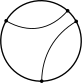
\includegraphics[width=0.115\textwidth]{graphics/four_term_from_stu_north.pdf}}
		\ - \
		\adjustbox{valign=c}{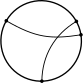
\includegraphics[width=0.115\textwidth]{graphics/four_term_from_stu_south.pdf}}
		\ = \
		\adjustbox{valign=c}{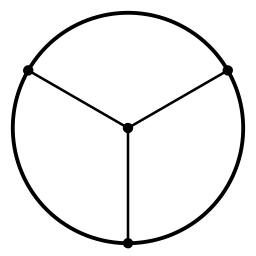
\includegraphics[width=0.12\textwidth]{four_term_jacobi_diagram.pdf}}
		\ = \
		\adjustbox{valign=c}{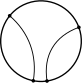
\includegraphics[width=0.115\textwidth]{graphics/four_term_from_stu_west.pdf}}
		\ - \
		\adjustbox{valign=c}{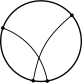
\includegraphics[width=0.115\textwidth]{graphics/four_term_from_stu_east.pdf}}\ .
	\]

\begin{definition}
	The algebra \(\mathcal{J}\) of Jacobi diagrams is the vector space \(\mathcal{T} / \ref{eq:STU}\), with the product \(\connect\) defined the same way as it was for chord diagrams.
\end{definition}

This is well-defined. The proof of Proposition \ref{prop:connected-sum-well-defined} showed that the product \(\connect\) being well-defined on \(\mathcal{A}\) was a consequence of the \ref{eq:4T} relations, which are implied by the \ref{eq:STU} relations. From the \ref{eq:STU} relations, we may deduce the following other relations which hold in \(\mathcal{J}\).

\begin{proposition}
	The following relations are consequences of the \textup{\ref{eq:STU}} relation in \(\mathcal{J}\):
	\begin{enumerate}
		\item The \textbf{AS relation} (antisymmetry relation),
			\begin{equation}
				\label{eq:AS}
				\tag{\as}
				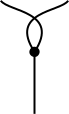
\includegraphics[width=0.05\textwidth, valign=c]{graphics/as_relation_a.pdf}
				\quad
				=
				\quad
				-
				\includegraphics[width=0.05\textwidth, valign=c]{graphics/as_relation_s.pdf}.
			\end{equation}
		\item The \textbf{IHX relation},
			\begin{equation}
				\label{eq:IHX}
				\tag{\ihx}
				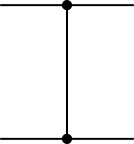
\includegraphics[width=0.10\textwidth, valign=c]{graphics/ihx_relation_i.pdf}
				\quad
				=
				\quad
				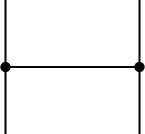
\includegraphics[width=0.10\textwidth, valign=c]{graphics/ihx_relation_h.pdf}
				\quad
				-
				\quad
				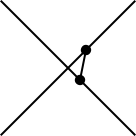
\includegraphics[width=0.10\textwidth, valign=c]{graphics/ihx_relation_x.pdf}.
			\end{equation}
	\end{enumerate}
\end{proposition}

\begin{proof}
	% TODO: Maybe put some images here.
	\begin{enumerate}
		\item
			Take two diagrams which differ only by \ref{eq:AS} at one (trivalent) vertex. If the vertex at which the \ref{eq:AS} relation resides is adjacent to a univalent vertex (i.e. touches the outer circle), then this is immediate from applying \ref{eq:STU} to both diagrams at that vertex.

			If the vertex is not immediately adjacent to a univalent vertex, then it is some \(d\) vertices `in the way'. By applying \ref{eq:STU} to those vertices yields a sum of \(2^{d}\) diagrams, all identical except for differing by \ref{eq:AS}, now on a vertex adjacent to a univalent vertex.

		\item
			A similar argument applies. If one of the two vertices of the \ref{eq:IHX} is adjacent to the circle, then the result is a direct consequence of an \ref{eq:STU} on each of the vertices. Otherwise, some \ref{eq:STU}s may be required first.
\end{enumerate}
\end{proof}

Looking at the relations \ref{eq:STU}, \ref{eq:AS} and \ref{eq:IHX}, the first solid evidence of Lie-theoretic structure in this story emerges. Explicit connections will be the subject of the next subsection, but for now notice that interpreting the trivalent vertex in \ref{eq:STU} (which has two `input' edges above and one `output' edge below) as a bracket, this bears resembelance to the relation that defines the universal enveloping algebra of a Lie algebra \([x, y] = xy - yx\). Similarly, \ref{eq:AS} looks like the antisymmetry property of the bracket \([x, y] = -[y, x]\). For \ref{eq:IHX} perhaps the relation isn't quite so obvious until the diagrams are rearranged into the form
\begin{equation*}
	\tag{\ihx}
	\includegraphics[width=0.10\textwidth, valign=c]{graphics/ihx_jacobi_form_i.pdf}
	\quad
	=
	\quad
	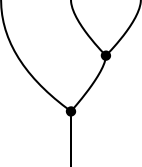
\includegraphics[width=0.10\textwidth, valign=c]{graphics/ihx_jacobi_form_h.pdf}
	\quad
	+
	\quad
	\includegraphics[width=0.10\textwidth, valign=c]{graphics/ihx_jacobi_form_x.pdf},
\end{equation*}
(here also one application of \ref{eq:AS} was used) whereby the \ref{eq:IHX} looks like the Jacobi identity, in the form \([[x, y], z] = [x, [y, z]] + [y, [x, z]]\).

% TODO: The change of basis assumption here is a liiitle sus.
We have already spoiled the surprise that in the end, \(\mathcal{A}\) and \(\mathcal{J}\) will be isomorphic as bialgebras. In fact, as algebras, this is clearly true so far, as \(\mathcal{J}\) is just a change of basis from \(\mathcal{A}\). Since \(\mathcal{A}\) spans \(\mathcal{J}\), we can attempt to lift the coproduct from \(\mathcal{A}\) directly onto \(\mathcal{J}\).

\begin{proposition}
	The coproduct \(\Delta\) on \(J \in \mathcal{J}\) defined by taking a Jacobi diagram, representing it as a chord diagram via \textup{\ref{eq:STU}}, taking the coproduct in \(\mathcal{A}\), then interpreting the result as a Jacobi diagram via the inclusion of \(\mathcal{A}\) into \(\mathcal{J}\), is also given by the following formula.

	\[\Delta(J) = \sum_{C \subset S} J_{C} \otimes J_{\overline{C}},\]
	where \(S\) is the set of connected components of \(J\), and \(\overline{C} = S \smallsetminus C\).
\end{proposition}

\begin{proof}
	Note that this has the same symbolic form as the coproduct in \(\mathcal{A}\) given in Definition~\ref{def:coproduct-in-chord-diagrams}, but with chords replaced by connected components of Jacobi diagrams. However, when working in \(\mathcal{A} \subset \mathcal{J}\), there are only univalent vertices, so the connected components are exactly the chords. Since \(\mathcal{A}\) forms a basis for \(\mathcal{J}\), and the formula is linear, it extends to all of \(\mathcal{J}\).
\end{proof}

\begin{corollary}
	The bialgebras \(\mathcal{A}\) and \(\mathcal{J}\) are isomorphic.
\end{corollary}

\begin{warning}
	From here on, justified by this isomorphism which is just a change of basis, we write \(\mathcal{J} = \mathcal{A}\), and \(\mathcal{A}\) is the preferred choice of notation for both chord diagrams and Jacobi diagrams.
\end{warning}

\section{Lie algebra weight systems}

\section{Non-Lie algebraic weight systems}

\section{Jacobi diagrams as a universal enveloping algebra}
